\paragraph{QuizziPedia::Front-End::Models::LangModel}
		
		\label{QuizziPedia::Front-End::Models::LangModel}
		
		\begin{figure}[ht]
			\centering
			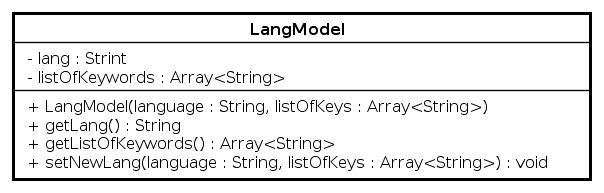
\includegraphics[scale=0.5,keepaspectratio]{UML/Classi/Front-End/QuizziPedia_Front-end_Models_LangModel.png}
			\caption{QuizziPedia::Front-End::Models::LangModel}
		\end{figure} \FloatBarrier
		
		\begin{itemize}
			\item \textbf{Descrizione}: rappresenta le informazioni per la giusta traduzione dell'applicazione;
			\item \textbf{Utilizzo}: viene utilizzata per racchiudere tutte le informazioni riguardanti la giusta traduzione dell'applicazione;
			\item \textbf{Relazioni con altre classi}: 
			\begin{itemize}
				\item \textbf{IN} \texttt{AppRun}: questa classe si preoccupa di creare la prima istanza dell'applicazione.
			\end{itemize}
			\item \textbf{Attributi}: 
			\begin{itemize}
				\item \texttt{- lang: String} \\
				Questo attributo rappresenta la lingua con il quale il sistema verrà visualizzato;  
				\item \texttt{- listOfKeywords: Array<String>} \\
				Questo attributo è un array di String che contiene il set di parole chiave che compongono la struttura dell'applicazione, necessarie per la traduzione delle pagine.
			\end{itemize}
			\item \textbf{Metodi}: 
			\begin{itemize}
				\item \texttt{+ LangModel(language: String, listOfKeys: Array<String>)} \\
				Metodo costruttore della classe.\\
				\textbf{Parametri}:
				\begin{itemize}
					\item {language: String}\\
					Questo parametro rappresenta la lingua con il quale il sistema verrà visualizzato;
					\item {listOfKeys: Array<String>}\\
					Questo parametro è un array di String che contiene il set di parole chiave che compongono la struttura dell'applicazione, necessarie per la traduzione delle pagine. 
				\end{itemize}
				
				\item \texttt{+ getLang(): String} \\
				Metodo che ritorna la lingua del sistema;
				
				\item \texttt{+ getListOfKeywords(): Array<String>} \\
				Metodo che ritorna la lista delle keywords nella lingua corrente del sistema;
				
				\item \texttt{+ setNewLang(language: String, listOfKeys: Array<String>): void} \\
				Metodo che setta la giusta lingua e la lista delle keywords.\\
				\textbf{Parametri}:
				\begin{itemize}
					\item {language: String}\\
					Questo parametro rappresenta la lingua con il quale il sistema verrà visualizzato;
					\item {listOfKeys: Array<String>}\\
					Questo parametro è un array di String che contiene il set di parole chiave che compongono la struttura dell'applicazione, necessarie per la traduzione delle pagine.
				\end{itemize}
				
			\end{itemize}
		\end{itemize}
		
		